\chapter{Fallbeispiel}
In diesem Kapitel werden die Erkenntnisse aus den beiden vorangehenden Kapiteln genutzt um das Poisson Problem $\Delta u = 1, u|_{\p \Omega} = 0$ auf einem L-förmigen Gebiet   
\[
\Omega = [0,1]^2 \cap \left\{ r(\cos\phi,\sin\phi)| r\in\R,0<\phi<\frac{3 \pi}{2} \right\}
\] 
zu approximieren, also mithilfe des Lösen-Approximieren-Markieren-Verfeinern Verfahren angewendet auf eine Anfangstriangulierung zusehen in Abbildung \ref{grid}.
\begin{figure}[!htbp]
	\begin{center}
		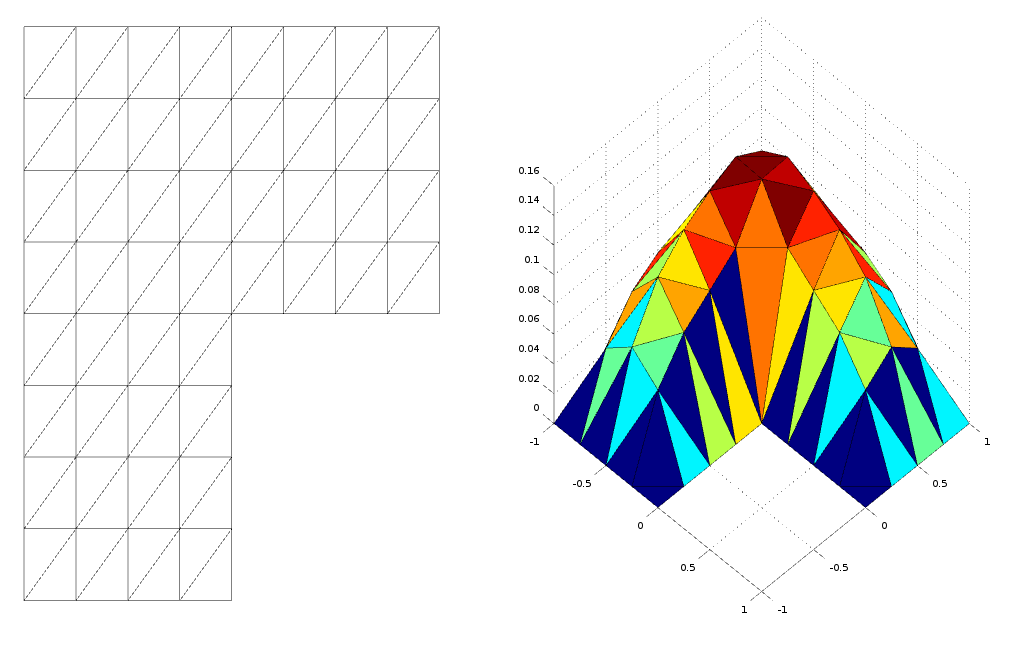
\includegraphics[width=15cm]{pics/nonref.png}
	\end{center}
	\caption{\label{grid}Triangulierung eines L-förmigen Gebiets (links) Approximierung einer Lösung des Poissonproblems (rechts)}
\end{figure}
\section{Implementation}
\begin{figure}
	\lstinputlisting{codes/p1_adaptive.m}
	\caption{ Hauptprogramm des Lösen-Approximieren-Markieren-Verfeinern Verfahrens (oben) Konstruktion der Finite Elemente Verfahrensmatrix (unten)}
\end{figure}

\begin{figure}
	\lstinputlisting{codes/p1_adaptive3.m}
	\caption{Berechnung der Verfeinerungsindikatoren}
\end{figure}

\begin{figure}
	\lstinputlisting{codes/p1_adaptive2.m}
	\caption{ \matlab-Implementation der Rot-Grün-Blau Verfeinerung}
\end{figure}

